We transition from presenting inference algorithms to applying them in practice. In the following chapter, we frame measuring student ability as an inference challenge, and leverage many of the same tools from previous chapters to handle the complexity of real world student cognition.

\section{Preliminaries}
\label{sec:introduction}

The task of estimating human ability from stochastic responses to a series of questions has been studied since the 1880's \cite{edgeworth1888statistics}
%%bd goes back way further! see, for example, Stable URL: http://www.jstor.org/stable/2339898
%%mw fixed
in thousands of papers spanning several fields.
The standard statistical model for this problem, Item Response Theory (IRT), is used every day around the world, in many critical contexts including college admissions tests, school-system assessment, survey analysis, popular questionnaires, and medical diagnosis.
As datasets become larger, new challenges and opportunities for improving IRT models present themselves.
On the one hand, massive datasets offer the opportunity to better understand human behavior by fitting more expressive models.
On the other hand, the algorithms that work for fitting small datasets often become intractable for larger data sizes.
% Indeed, despite a large body of literature, contemporary IRT methods fall short -- it remains surprisingly difficult to estimate human ability from stochastic responses. 
%%bd says who? i am not just being a pedant but am not entirely sure what we mean. i think most psychometrics people would say that merely getting estimates isnt that big of a challenge at this stage. i would suggest we try to refine to more clealry indicate the problem we care about. to my mind, that is a typical reliance on highly parametric models required to do inference given the latent variables (ie ability) that make estimation complex here.
%% mw: @ben, this is a good point! I am going to focus this paragraph on just the scalability argument and bring up this parametric argument later for the deep generative IRT parts
One crucial bottleneck is that the most accurate, state-of-the-art Bayesian inference algorithms are prohibitively slow, while faster algorithms (such as the popular maximum marginal likelihood estimators) sacrifice accuracy with simplifying assumptions and poorly capture uncertainty.
This leaves practitioners with a choice: either have nuanced Bayesian models with appropriate inference or have timely computation.

In the field of artificial intelligence, a revolution in deep generative models via \emph{variational inference} \cite{kingma2013auto,rezende2014stochastic} has demonstrated an impressive ability to perform fast inference for complex Bayesian models.
In this paper, we present a novel application of variational inference to IRT, validate the resulting algorithms with synthetic datasets, and apply them to real world datasets.
We then show that this inference approach allows us to extend classic IRT response models with deep neural network components. We find that these more flexible models better fit large real world datasets.
Specifically, our contributions are as follows:

\begin{enumerate}
    \item \textbf{Variational inference for IRT:} We derive a new optimization objective --- the Variational Item response theory Lower Bound, or VIBO --- to perform inference in IRT models.
    By learning a mapping from responses to posterior distributions over ability and items, VIBO is 
    trained to efficiently solve many inference queries at once; a process called \textit{amortization}.
    %bd this word is a mystery to me. can we parenthetically help reader here?
    %mw: great point. is this better?
    \item \textbf{Faster inference:}
    We find VIBO to be much faster than previous Bayesian techniques and usable on much larger datasets without loss in accuracy.
    \item \textbf{More expressive:} Our inference approach is naturally compatible with deep generative models: we train neural networks to learn a joint mapping from student ability and item characteristics to response probabilities. As universal function approximators, neural networks capture nonlinear mappings that are more flexible than commonly used parametric IRT models (e.g. 2PL or LPE).
    % and, thus, we extend Bayesian IRT models to use neural-network-based representations for inputs, predictions, and student ability. 
    %%bd i'm not clear on what inputs and predictsion mean in this context
    %% mw: fixed.
    To the best of our knowledge, we are the first to apply deep generative models to IRT. %%bd i am always hesitant to include claims of primacy as they basically serve as a dare for some wacky reviewer to prove you wrong. but, if you're sure it's right... :)
    %% mw: i want to be a little bold here and try to claim this contribution. We can retract if we get a lot of pushback!
    % \item \textbf{Simple code:} We open-sourced both a Python pip package (TODO) and a CRAN R package (TODO), inspired by MIRT, to make VIBO accessible for practitioners.
    We leverage this flexibility to uncover asymmetric item characteristic curves from data alone, and show examples on the TIMSS dataset.
    \item \textbf{Real world application: } We demonstrate the impact of faster inference and expressive models by applying our algorithms to datasets of responses from PISA, DuoLingo and Gradescope. We achieve up to 200 times speedup relative to conventional parametric approaches and show improved accuracy at imputing hidden responses.
    At scale, these improvements in efficiency save hundreds of hours of computation.
    % \item \textbf{Learning item characteric curves:} We show how to use VIBO to uncover asymmetric item characteristic curves from data alone---an example motivated by recent work in the psychometrics literature---and show examples using the TIMSS dataset. \ndg{this should really be part of point 3 -- we extend the generative model first in constrained ways, such as learning the characteristic curves, and then by replacing the classical generative model with a deep network.}
\end{enumerate}

As a roadmap, in the following sections, we first describe the item response theory challenge before we present the main algorithm. Then, through experiments on several measurement datasets, we show its impact on speed and accuracy.
We discuss several extension to the IRT generative model, made possible by the VIBO algorithm: handling polytomous responses, capturing asymmetric item characteristic curves, and using flexible deep generative models. We close with limitations and broader impact of the proposed method.
% The potential impact of this work is two-fold: More accurate models can be constructed for existing applications of Item Response Theory, such as for visual acuity tests (Piech, 2019), large scale language studies (Hartshorne, 2018), or educational assessments such as PISA (Organisation, 2016).

\section{Preliminaries}
\label{sec:background}

We briefly review several variations of IRT and the fundamental principles of approximate Bayesian inference, focusing on stochastic variational inference.
A visualization of the different item response functions discussed can be found in Figure~\ref{fig:icc}.
%%bd suggest we add: We discuss several item response models; a visualization of the item response functions invoked by these models can be found in Figure X.

\begin{figure}
    \centering
    \includegraphics[width=0.6\textwidth]{images/chapter7/icc.pdf}
    \caption{Item characteric curves (ICC) for various IRT models. IDL represents an ideal point model (non-monotonic); LPE represents a logistic positive exponent model (asymmetric). For 3PL, we set the guess parameter $g_j = 0.3$. For LPE, we vary $b_j = 0.3$ and $b_j = 3.0$.}
    \label{fig:icc}
\end{figure}

% Imagine answering a series of multiple choice questions.
% For example, consider a personality survey, a homework assignment, or a school entrance examination.
% Selecting a response to each question is an interaction between your ``ability'' (knowledge or features) and the characteristics of the question, such as its difficulty.
% The goal in examination analysis is to gauge this unknown ability of each student and the unknown item characteristics based only on responses.
% Early procedures (Edgeworth, 1888) defaulted to very simple methods, such as counting the number of correct responses, which ignore differences in question quality.
% In reality, we understand that not all questions are created equal: some may be hard to understand while others may test more difficult concepts.
% To capture these nuances, Item Response Theory (IRT) was developed as a mathematical framework to reason jointly about people's ability and the items themselves.

% The IRT model plays an impactful role in many large institutions.
% It is the preferred method for estimating ability in several state assessments in the United States, for international assessments gauging educational competency across countries (Harlen, 2001), and for the National Assessment of Educational Programs (NAEP), a large-scale measurement of literacy and reading comprehension in the US (Ravitch, 1995).
% Beyond education, IRT is widely used in cognitive science and psychology, for instance, to study  language acquisition and development (Hartshorne, 2018; Magdalena, 2016; Frank, 2017; Braginsky, 2015).
Item response theory (IRT) is widely used to model the probability of a correct response conditional on a latent set of ``abilities'' and item characteristics, with applications in educational assessment \cite{edgeworth1888statistics,ravitch1995national,harlen2001assessment}, language development \cite{braginsky2015developmental,luniewska2016ratings,frank2017wordbank,hartshorne2018critical}, and many other areas.

\begin{figure}
    \centering
    \begin{subfigure}[b]{0.3\textwidth}
        \centering
        \includegraphics[width=0.75\textwidth]{images/chapter7/irt_1pl.pdf}
        \caption{}
    \end{subfigure}
    \begin{subfigure}[b]{0.3\textwidth}
        \centering
        \includegraphics[width=0.75\textwidth]{images/chapter7/irt_2pl.pdf}
        \caption{}
    \end{subfigure}
    \begin{subfigure}[b]{0.3\textwidth}
        \centering
        \includegraphics[width=0.75\textwidth]{images/chapter7/irt_3pl.pdf}
        \caption{}
    \end{subfigure}
    \caption{Graphical models for the (a) 1PL, (b) 2PL, and (c) 3PL Item Response Theories. Observed variables are shaded. Arrows represent dependency between random variables and each rectangle represents a plate (i.e.~repeated observations).}
    \label{fig:irt_graph}
\end{figure}

%%bd i think we could probably delete the stuff in the section ahead of this as it should be highly familiar to journal's readership. we could add a first sentence saying ``IRT is widely used to model the probability of a response conditional on some latent set of ``abilities'' (then add cites)''
%%mw: done.
IRT has taken many forms over it's rich history. As review, we begin with the most standard (see Figure~\ref{fig:irt_graph}).
The simplest class of IRT summarizes the ability of a person with a single parameter.
This class contains three versions: 1PL, 2PL, and 3PL -IRT, each of which differ by the number of free variables used to characterize an item.
The 1PL-IRT model, also called the Rasch model \cite{rasch1960studies}, is given in Equation~\ref{eq:1pl_irt},
\begin{equation}
    p(r_{i,j}=1|a_i,d_j) = \frac{1}{1 + e^{-a_i - d_j}}
\label{eq:1pl_irt}
\end{equation}
where $r_{i,j}$ is the response by the $i$-th person to the $j$-th item.
There are $N$ people and $M$ items in total.
Each item in the 1PL model is characterized by a single number representing difficulty, $d_j$.
%%As the 1PL model is equivalent to a logistic function, a higher difficulty requires a higher ability in order to respond correctly.
The 2PL-IRT model adds a \textit{discrimination} parameter, $k_j$ for each item that controls the slope (or scale) of the item response function. 
%%bd if you accept edit above re the logistic function line, i think you could just talk about k_j controlling slope of resulting item response function. in fact, it might be useful to introduce the item response function as the key thing we're focusing on here (eg when we say 'accuracy' we mean accurate estimation of that function)
%% mw: changed logistic -> item response function. Will try to mention item response functions in the evaluation section. I think too early to mention here.
Items with higher discrimination to more quickly separate people of low and high ability.
The 3PL-IRT model further adds a \textit{pseudo-guessing} parameter, $g_j$ for each item that sets the asymptotic minimum of the item response function.
We can interpret pseudo-guessing as the probability of success if the respondent were to make a (reasonable) guess on an item.
The 2PL and 3PL -IRT models, respectively, are:
\begin{equation}
   p(r_{i,j}|a_i, k_j, d_j) = \frac{1}{1 + e^{-k_j a_i - d_j}} \textup{ or } p(r_{i,j} | a_i, g_j, k_j, d_j) = g_j + \frac{1 - g_j}{1 + e^{-k_j a_i - d_j}}
\label{eq:2and3pl_irt}
\end{equation}
See Figure~\ref{fig:irt_graph} for graphical models of each of these IRT models where arrows represent conditional dependencies. 
% `Below, we may write $\textbf{d}_j = \{k_j, d_j\}$ or $\textbf{d}_j = \{g_j, k_j, d_j\}$ to represent the set of item characteristics. 

\subsubsection{Multidimensional Extensions}

While ability and item characteristics presented above are scalars, later extensions proposed more flexible IRT models using multi-dimensional representations of ability and item discrimination \cite{ackerman1994using,mcdonald2000basis,reckase2009multidimensional}.
However, in return for flexibility, multi-dimensional IRT (or MIRT) is computationally cumbersome, requiring expensive numerical quadratures \cite{liu1994note,naylor1982applications} or MCMC sampling \cite{houts2015flexmirt}  to perform inference. 
% A single ability dimension is sometimes insufficient to capture the relevant variation in human responses.
% For instance, if we are measuring a person's understanding on elementary arithmetic, then a single dimension may suffice in capturing the majority of the variance.
% However, if we are instead measuring a person's general mathematics ability, a single real number no longer seems sufficient.
% Even if we bound the domain to middle school mathematics, there are several factors that contribute to ``mathematical understanding" (e.g. proficiency in algebra versus geometry).
% Summarizing a person with a single number in this setting would result in a fairly loose approximation.
%%bd i would probably steer clear of this kind of example. i don't personally find it objectionable, but it could be the kind of thing that a MD irt person has strong feelings about. i think we could probably just excise the stuff above this comment and then maybe note that adding flexibility to these models is hugely computationally cumbersome (to my mind, it wasn't even really until li cai's work that came out when i was in grad school that this became possible. that might be a good cite given that it was in psychometrika: https://link.springer.com/content/pdf/10.1007/s11336-009-9136-x.pdf
% mw: great point. Fixed.
% For cases where multiple facets of ability contribute to performance, we consider \textit{multidimensional} item response theory (Ackerman, 1994; Reckase, 2009; Mcdonald, 2000).
More explicitly, the multidimensional extension to 2PL-IRT can be expressed as:
\begin{equation}
    p(r_{i,j}=1|\textbf{a}_i, \textbf{k}_j, d_j) = \frac{1}{1 + e^{-\textbf{a}_i^T \textbf{k}_j - d_j}}
\label{eq:3pl_mirt}
\end{equation}
where we overload notation $\textbf{a}_i = \left(a^{(1)}_i, a^{(2)}_i, \ldots, a^{(K)}_i\right)$ to represent a $K$ dimensional vector. Similarly, the item discrimination $\textbf{k}_j = \left(k^{(1)}_i, k^{(2)}_i, \ldots, k^{(K)}_i\right)$ becomes a vector of equal dimensionality to ability.

Despite the increased expressivity of moving to multidimensional representations, MIRT still assumes a linear relationship between ability and item characterics, which has its limitations in real world applications. As such, IRT research has shifted towards injecting ``non-linearity'' in the traditional IRT model, starting with extensions using nonlinear response functions.
% \ndg{i think it'd be good to put a sentence or two pointing out that this linear "compensatory" relationship between dimensions has limitations, and many people have explored other forms. (it's good to set this up because it's part of the reason the fullly deep generative version is worth exploring...)}
% mw: yeah great call.

\subsubsection{Asymmetric Extensions}

Almost all of the IRT models presented thus far have symmetric item characteristic curves (ICCs), meaning that there exists an inflection point in ability such that any increase in ability beyond the inflection point results in a change in probability (of answering an item correctly) that is mirrored by an equivalent decrease in ability below the inflection point.
The 3PL breaks this symmetry, as it introduces a ``guessing'' hyperparameter that applies a floor to the left half of the ICC. 
However, there are more sophisticated ways to introduce asymmetries. 

The logistic positive exponent IRT model, or LPE \cite{samejima2000logistic} presents one way. It introduces a third item parameter that represents a psychometric notion of ``complexity'' that captures the number of conjunctively or disjunctively interacting subprocesses, i.e., ``cognitive steps'', required for the item. The LPE-IRT model has the following unidimensional form:
\begin{equation}
    p(r_{i,j}|a_i, k_j, d_j, b_j) = \left(\frac{1}{1 + e^{-k_j a_i - d_j}}\right)^{b_j}.
\label{eq:lpe_mirt}
\end{equation}
If the complexity term $b_j = 1$, the ICCs are symmetric, and LPE collapses to 2PL-IRT. When $0 < b_j < 1$, the ICC would accelerate at a faster rate to the right of the inflection point than to the left, representing disjunctively interacting subprocesses. When $b_j > 1$, the ICC would accelerate at a slower rate to the right of the inflection point than to the right, representing conjunctively interacting subprocesses. 
See Figure~\ref{fig:icc} for a visualization of the ICCs. 
%%bd this should probably be figure 2, yeah? also, i would maybe note that we have such item response functions for all the models you talk about in this section. perhaps something to say at the outset of section (will add comment there)
%%mw: why figure 2? 
% \ndg{maybe note the connection between LPE and non-compensatory mirt?}
In $K$ dimensions, if we let $b_j = K$ and assume isometric ability and item discrimination, the LPE model is equivalent to non-compensatory MIRT \cite{sympson1978model,ackerman1989unidimensional}.
While LPE and the more general non-compensatory model capture different interactions than its compensatory cousins (e.g. 2PL-MIRT), it is not clear when to use which model. 
An open problem remains to leverage student responses to infer which model is most appropriate.
% \mwu{don't know to use AND or OR.}

\subsubsection{Non-Monotonic Extensions}

Fundamental to IRT models we have seen so far (including asymmetric ones) is the assumption that higher ability results in higher response scores.
However, in complex real-world settings, this may not be a good assumption. Rather scores may vary non-monotonically with respect to the underlying latent trait.
With this as motivation, \textit{unfolding} models were proposed as a non-monotonic extension of IRT, where the response is defined by a nonlinear distance between the individual ability and item difficulty.
Critically, this nonlinearity implies that purely higher ability does not necessarily suggest higher response scores.

In this paper, we will study ideal point IRT models \cite{maydeu2006multidimensional}, abbreviated as IDL or MIDL in the multi-dimensional case.
In one dimension, the item response function is:
\begin{equation}
    p(r_{i,j}=1|a_i,k_j,d_j) = e^{-\frac{1}{2}(-k_j a_i - d_j)^2} 
\end{equation}
or in multi-dimensions:
\begin{equation}
    p(r_{i,j}=1|\textbf{a}_i,\textbf{k}_j,d_j) = e^{-\frac{1}{2}(-\textbf{k}_j^T \textbf{a}_i - d_j)^2}
\end{equation}
where $\textbf{a}_i$, $\textbf{k}_j$, and $d_j$ are as defined in traditional IRT. Note that the form of IDL is closely related to a Gaussian PDF.
In particular, the squared term results in the non-monotonicity of the response function.

\subsection{Inference in Item Response Theory}

In practice, we are interested in solving an \textit{inference} task. Given a (possibly incomplete) $N \times M$ matrix of observed responses, we want to \textit{infer} the ability of all $N$ people and the characteristics of all $M$ items.
More generally, inference is the task of estimating unknown variables, such as ability or item characteristics, given observations, such as student responses. We compare and contrast  three popular methods used to perform inference for IRT in research and industry. Inference algorithms are critical for item response theory as slow or inaccurate algorithms prevent the use of appropriate models. In the exposition below, we assume a unidimensional 2PL IRT model with no loss of generality.

\subsubsection{Maximum Likelihood Estimation}
A straightforward approach is to pick the most likely ability and item features given the observed responses.
To do so we optimize:
\begin{align}
    L_{\textup{MLE}} &= \max_{\{a_i\}_{i=1}^N, \{d_j, k_j\}_{j=1}^M} \sum_{i=1}^N \sum_{j=1}^M \log p(r_{i,j}|a_i, d_j, k_j)
    \label{eqn:jmle}
\end{align}
with stochastic gradient descent (See e.g. \cite{Goodfellow-et-al-2016}). A similar definition as to Equation~\ref{eqn:jmle} can be written for 1PL and 3PL models. 
Equation~\ref{eqn:jmle} is often called the Joint Maximum Likelihood Estimator \cite{beguin2001mcmc,beguin2001mcmc,chen2019joint}, abbreviated JMLE. 
JMLE poses inference as a supervised regression problem in which we choose the most likely unknown variables to match known dependent variables.
While JMLE is simple to understand and implement, it lacks any measure of uncertainty; this can have important consequences when responses are missing.

\subsubsection{Expectation Maximization}
Several papers have noted that when using JMLE, the number of unknown parameters increases with the number of people \cite{bock1981marginal,haberman1977maximum}.
In particular, \cite{haberman1977maximum} shows that in practical settings with a finite number of items, standard convergence theorems do not hold for JMLE as the number of people grows.
To remedy this, the authors instead treat ability as a nuisance parameter and marginalized it out \cite{bock1981marginal,bock1988full}.
\cite{dempster1977maximum} introduces an Expectation-Maximization (EM) algorithm to iterate between (1) updating beliefs about item characteristics and (2) using the updated beliefs to define a marginal distribution (without ability) $p(r_{i,j}|k_j, d_j)$ by numerical integration of $a_i$.
Appropriately, this algorithm is referred to as Maximum Marginal Likelihood Estimation, which we abbreviate as EM.
Equation~\ref{eqn:em} shows the E and M steps for EM.
\begin{align}
    \textup{E step}:&\quad p(r_{i,j}|d^{(t)}_j, k^{(t)}_j) = \int_{a_i} p(r_{i,j}|a_i, d^{(t)}_j, k^{(t)}_j)p(a_i) d a_i \\
    \textup{M step}:&\quad \{d_j^{(t+1)}, k_j^{(t+1)}\} = \arg\max_{d_j} \sum_{i=1}^N \log p(r_{i,j} |d^{(t)}_j, k^{(t)}_j)
    \label{eqn:em}
\end{align}
where the superscript $(t)$ represents the iteration count.
We choose $p(a_i)$ to be a simple prior distribution like standard Normal.
In general, the integral in the E-step is intractable.
EM uses a Gaussian-Hermite quadrature to discretely approximate $p(r_{i,j}|d^{(t)}_j,k^{(t)}_j)$.
See \cite{harwell1988item} for a closed form expression for the optimal parameters $\{d_j^{(t+1)}, k_j^{(t+1)}\}$ in the M step.
This method finds the maximum a posteriori (MAP) estimate for item characteristics.
Note EM does not infer ability as it is ``ignored" in the model: the common workaround is to use EM to infer item characteristics, then estimate ability by fitting a second auxiliary model.
In practice, EM has grown to be ubiquitous in industry as it is incredibly fast for small to medium sized datasets.
However, we expect that EM may scale poorly to large datasets with many items and higher dimensions (e.g. replace $a_i$ with $\textbf{a}_i$) as numerical integration requires far more points to properly measure a high dimensional volume.
One of our goals is to propose a new method that is as fast as EM but also scalable.

\subsubsection{Hamiltonian Monte Carlo}
The two inference methods above give only point estimates for ability and item characteristics.
In contrast Bayesian approaches seek to capture the full posterior over ability and item characteristics given observed responses, $p(a_{1:N},d_{1:M},k_{1:M}|r_{1:N,1:M}) = \prod_{i=1}^N p(a_i,d_{1:M},k_{1:M}|r_{i,1:M})$ where $r_{i,1:M} = (r_{i,1}, \cdots, r_{i,M})$ are the $i$-th individual's responses to $M$ items. 
% \ndg{shouldn't this be $a_{1:N}$?}
% mw: see edit.
Doing so provides estimates of uncertainty and characterizes features of the joint distribution that cannot be represented by point estimates, such as multimodality and parameter correlation.
In practice, this can be very useful for a more robust understanding of student ability.

The common technique for Bayesian estimation in IRT uses Markov Chain Monte Carlo, or MCMC \cite{hastings1970monte, gelfand1990sampling} to draw samples from the posterior by constructing a Markov chain carefully designed such that $p(a_i,d_{1:M}|r_{i,1:M})$ is the equilibrium distribution.
By running the chain longer, we can closely match the distribution of drawn samples to the true posterior distribution.
Hamiltonian Monte Carlo, or HMC \cite{neal2011mcmc, neal1994improved, hoffman2014no} is an efficient version of MCMC for continuous state spaces that leverages gradient information.
We recommend \cite{hoffman2014no} for a good review of MCMC and HMC.

The strength of this approach is that the samples generated capture the true posterior (if the algorithm is run long enough).
But the computational costs for MCMC can be very high, and the cost scales at least linearly with the number of latent parameters --- which for IRT is proportional to data size.
With new datasets of millions of observations, such limitations can be debilitating.
Fortunately, there exist a second class of approximate Bayesian techniques that have gained significant traction in the machine learning community, called \textit{variational inference}.
% We provide a careful review of modern variational inference.

\section{The VIBO Algorithm}
\label{sec:methods}
Having introduced the major principles of VI, we will adapt them to IRT.
In our review, we presented the ELBO that serves as the primary loss function to train an inference model. Given the nuances of IRT, we can derive a new loss function specialized for ability and item characteristics. We call the resulting algorithm VIBO since it is a \textbf{V}ariational approach for \textbf{I}tem response theory based on a novel lower \textbf{BO}und.
While the remainder of the section presents the technical details, we ask the reader to keep the high-level purpose in mind: VIBO is an objective function that if we maximize, we have a method to predict student ability and item characteristics with confidences from a student's responses. As a optimization problem, VIBO is much cheaper computationally than MCMC.

To show that doing so is justifiable, we prove that VIBO well-defined. That is, we must show that VIBO lower bounds the marginal likelihood over a student's responses. By doing so, we show that maximizing this bound will minimize the divergence between our approximate posteriors over ability and item characteristics, and the true posterior.
In other words, maximizing VIBO ensures better inference of IRT parameters.
Like above, we present VIBO for unidimensional 2PL IRT but note no restrictions to higher dimensions or other IRT families. 
% \ndg{should say more clearly why we need this... possibly move the theorem or at least its proof to an appendix??}

\begin{thm}
    Let $a_i$ be the ability for person $i \in [1, N]$ and $\{k_j,d_j\}$ be the characteristics for item $j \in [1, M]$. We use the shorthand notation $d_{1:M} = (d_1, \ldots, d_M)$ with a similar definition for $k_{1:M}$. Let $r_{i,j}$ be the binary response for item $j$ by person $i$. We write $r_{i, 1:M} = (r_{i,1}, \ldots r_{i,M})$.
    If we define the VIBO objective as:
    \begin{equation}
        \textup{VIBO}(r_{i,1:M}) = L_{\text{recon}} + \mathbf{E}_{q_\phi(d_{1:M},k_{1:M}|r_{i,1:M})}[D_{\text{ability}}] +D_{\text{item}}
        \label{eq:vibo:og}
    \end{equation}
    where
    \begin{align*}
        L_{\text{recon}} &= \mathbf{E}_{q_\phi(a_i, d_{1:M}, k_{1:M}|r_{i,1:M})}\left[ \log p_\theta(r_{i,1:M}|a_i, d_{1:M}, k_{1:M}) \right] \\
        D_{\text{ability}} &= \textup{KL}(q_\phi(a_i|d_{1:M},k_{1:M}, r_{i,1:M}), p(a_i)) \\
        D_{\text{item}} &= \textup{KL}(q_\phi(d_{1:M},k_{1:M}|r_{i,1:M})||p(d_{1:M}, k_{1:M})),
    \end{align*}
    and assume the joint posterior factors as 
    \begin{align}
        q_\phi(a_i, d_{1:M}, k_{1:M}|r_{i,1:M}) = q_\phi(a_i|d_{1:M},k_{1:M},r_{i,1:M})q_\phi(d_{1:M},k_{1:M}|r_{i,1:M}) \\
        q_\phi(d_{1:M},k_{1:M}|r_{i,1:M}) = q_\phi(d_{1:M}|r_{i,1:M})q_\phi(k_{1:M}|r_{i,1:M}) 
    \end{align}
    then $\log p(r_{i,1:M}) \geq \textup{VIBO}$. In other words, VIBO is a lower bound on the log marginal probability of student $i$'s responses.
    \label{thm:virtu}
\end{thm}

See Section~\ref{sec:proof:vibo} for a complete proof of Theorem~\ref{thm:virtu}.
The theorem leaves several choices up to us, and we opt for the simplest ones.
For instance, the prior distributions are chosen to be independent standard Normal distributions, $p(a_i) = \prod_{k=1}^K p(a_{i,k})$ and $p(d_{1:M}) = \prod_{j=1}^M p(d_{j})$ where $p(a_{i,k})$ and $p(d_j)$ are $N(0,1)$.
Further, we found it sufficient to assume 
\begin{equation}
    q_\phi(d_{1:M},k_{1:M}|r_{i,1:M}) = q_\phi(d_{1:M})q_\phi(k_{1:M})= \left(\prod_{j=1}^M q_\phi(d_{j})\right)\left(\prod_{j=1}^M q_\phi(k_{j})\right),
\end{equation}
meaning that the inference networks for item characteristics are not amortized. Further, the joint distribution over item parameters factors to independent marginals.
We emphasize that this factorization does not mean item characteristics are independent of responses as we still leverage response data to learn the best choices for $\{d_{1:M},k_{1:M}\}$ but we do not explicitly learn a mapping from response to item features. 
Future work can investigate amortizing item characteristics.
% \ndg{this will confuse people... item characteristics are not independent of responses since argmax of phi depends on data, but rather they are not amortized...}
Initially, we assume the generative model $p_\theta(r_{i,1:M}|a_i,d_{1:M})$ to be an IRT model (thus there are no trainable model parameters beyond the explicit item and ability parameters i.e. $\theta$ is empty); later we explore generalizations.

% \begin{algorithm}[h!]
% \SetAlgoLined
%     Assume we are given observed responses for person $i$, $\textbf{r}_{i1:M}$\;
%     Compute $\mu_{\textbf{d}}, \sigma^2_{\textbf{d}} = q_\phi(\textbf{d}_{1:M})$\;
%     Sample $\textbf{d}_{1:M} \sim N(\mu_{\textbf{d}}, \sigma^2_{\textbf{d}})$\;
%     Compute $\mu_{a}, \sigma^2_{a} = q_\phi(\textbf{a}_i|\textbf{d}_{1:M},\textbf{r}_{i,1:M})$\;
%     Sample $\textbf{a}_i \sim N(\mu_{a}, \sigma^2_{a})$\;
%     Compute $L_{\text{recon}} = \log p_\theta(\textbf{r}_{i,1:M}|\textbf{a}_i,\textbf{d}_{1:M})$\;
%     Compute $D_{\text{ability}} = \\textup{KL}(N(\mu_{a}, \sigma^2_{a})||N(0,1))$\;
%     Compute $D_{\text{item}} = \\textup{KL}(N(\mu_{\textbf{d}}, \sigma^2_{\textbf{d}})||N(0,1))$\;
%     Compute $\text{VIBO} = L_{\text{recon}} + D_{\text{ability}} + D_{\text{item}}$
%     \caption{VIBO Forward Pass}
%     \label{alg:vibo}
% \end{algorithm}

The posterior $q_\phi(a_i|d_{1:M},r_{i,1:M})$ needs to be robust to missing data as often not every person answers every question.
As a practical example, students taking the GRE are given different subsets of questions based on performance.
To achieve this, we explore the following family:
\begin{equation}
    q_\phi(a_i|d_{1:M},k_{1:M},r_{i,1:M}) = \prod_{j=1}^M q_\phi(a_i|d_j,k_j,r_{i,j})
\end{equation}
If we assume each component $q_\phi(a_i|d_j,k_j,r_{i,j})$ is Gaussian, then $q_\phi(a_i|d_{1:M},k_{1:M},r_{i,1:M})$ is Gaussian as well, being a Product-of-Experts \cite{hinton1999products,wu2018multimodal}.
If item $j$ is missing, we replace its term in the product with the prior, $p(a_i)$ representing no added information.
We found this product of experts design to outperform averaging over non-missing entries (i.e., experts with equal weighting): $q_\phi(a_i|d_{1:M},k_{1:M},r_{i,1:M}) = \frac{1}{M}\sum_{j=1}^M q_\phi(a_i|d_j,k_j,r_{i,j})$.
See Section~\ref{sec:app:vibo} for an experimental comparison as well as two other decompositions of $q_\phi(a_i|d_{1:M},k_{1:M},r_{i,1:M})$.

As VIBO is a close cousin of the ELBO, we can estimate its gradients similarly:
\begin{align*}
    \nabla_\theta \textup{VIBO}({r}_{i,1:M}) &= \nabla_\theta L_{\text{recon}} \\
    &= \mathbf{E}_{q_\phi({a}_i, {d}_{1:M}, k_{1:M}|{r}_{i,1:M})}\left[ \nabla_\theta \log p_\theta({r}_{i,1:M}|{a}_i, {d}_{1:M}, k_{1:M}) \right] \\
    \nabla_\phi \textup{VIBO}({r}_{i,1:M}) &= \nabla_\phi \mathbf{E}_{q_\phi({d}_{1:M}, k_{1:M}|{r}_{i,1:M})}[D_{\text{ability}}] + \nabla_\phi D_{\text{item}} \\
    &= \nabla_\phi \mathbf{E}_{q_\phi({a}_i,{d}_{1:M}, k_{1:M}|{r}_{i,1:M})}\left[\frac{p({a}_i)p({d}_{1:M})p(k_{1:M})}{q_\phi({a}_i,{d}_{1:M}, k_{1:M}|{r}_{i,1:M})}\right]
\end{align*}
As with the ELBO, we may wish to move the gradient inside the \textup{KL} divergences ($D_{\text{ability}}$ and $D_{\text{item}}$) by reparameterization to reduce variance.
To allow easy reparameterization, we define all variational distributions $q_\phi(\cdot|\cdot)$ as Normal distributions with diagonal covariance. 
We point that this choice does not constrain the joint distribution over ability and item characteristics to be Gaussian, as abilities are sampled conditional on item characteristics.
% \ndg{it would be useful to point out that this doesn't mean the parameters are jointly gaussian, since abilities are sampled conditional on item params....}
In practice, we find that estimating $\nabla_\theta \text{VIBO}$ and $\nabla_\phi \text{VIBO}$ with a single sample is sufficient.
With this setup, VIBO can be optimized using stochastic gradient descent to learn an amortized inference model that maximizes the marginal probability of observed data.
As done with the ELBO, we can optimize $\mathbf{E}_{{r}_{i,1:M} \sim p_{D}}\left[\text{VIBO}({r}_{i,1:M})\right]$ by i.i.d. sampling minibatches of $M$ responses from different individuals from a dataset $D$.
Using minibatches is crucial to scaling up to large datasets.
% We summarize the required computation to calculate VIBO in Algorithm~\ref{alg:vibo}.
% \ndg{somehow the fact that we sample minibatches of data points has slipped under the radar..}

\subsubsection{Beta Regularization}

The balance between terms in the ELBO is known to affect optimization stability \cite{higgins2016beta}.
We thus add a hyperparameter to scale the \textup{KL} divergence terms. That is, we write VIBO as:
\begin{equation}
    \textup{VIBO}({r}_{i,1:M}) = L_{\text{recon}} + \beta\mathbf{E}_{q_\phi({d}_{1:M}, k_{1:M}|{r}_{i,1:M})}[D_{\text{ability}}] + \beta D_{\text{item}}
    \label{eq:betareg}
\end{equation}
where $\beta > 0$ (by default, $\beta = 1$). In practice, $L_{\text{recon}}$ is dependent on the dimensionality and domain of the data.
If the magnitude of $L_{\text{recon}}$ greatly outweighs the \textup{KL} divergence terms, the posteriors will not be sufficiently regularized.
Likewise, if the magnitude of $L_{\text{recon}}$ is too small, inference will be inaccurate.
Choosing $\beta$ offers a way for the practitioner to balance the magnitudes. 
It is closely related to $\beta$-VAE (Higgins, 2016), although we do not study disentanglement effects in the latent variables.
In practice, we fix $\beta$ based on dimensionality $K$ and cross-validation.
% \ndg{don't we effectively fix beta based on dimensionality? say this is default?}

\subsubsection{Polytomous Responses}

Thus far, we have assumed that response data $r_{i,j}$ is either 0 or 1.
In practice, this assumption may not always be realistic. Many questionnaires and examinations are not binary: responses can be multiple choice (e.g. Likert scale) or even real valued (e.g. 92\% on a course test).
Fortunately, VIBO is flexible enough to model a more general class of responses. 
In Equation~\ref{eq:vibo:og}, we write the likelihood of the $j$-th response from the $i$-th person given their ability and item characteristics as $p_\theta(r_{i,j}|{a}_i, {d}_{j}, k_j)$. 
For binary responses, this distribution $p_\theta$ is parameterized as a Bernoulli distribution representing the likelihood of $r_{i,j}$ being correct. 
Yet nothing prevents us from choosing a different distribution, such as Categorical for multiple choice responses or Normal for real-values.
For example, suppose $r_{i,j}$ is real-valued. Then, the VIBO generative model could map ${a}_i$ and $\{{d}_{j}, k_j\}$ to a Gaussian distribution used to score the response, $r_{i,j}$. 
In our experiments, we will mostly study binary responses, but will explore continuous responses in a later subsection.

\section{Dataset Overview}
\label{sec:datasets}
We explore one synthetic dataset, to build intuition and confirm parameter recovery, and five large scale applications of IRT to real world data, summarized in Table~\ref{table:datasets}.

\begin{table}[h!]
    \caption{Dataset Statistics}
    \label{table:datasets}
    \begin{center}
    \begin{tabular}{lccc}
    \hline
    & \# Persons & \# Items & Missing Data? \\
    \hline
    CritLangAcq & 669498 & 95 & N \\
    WordBank & 5520 & 797 & N \\
    DuoLingo & 2587 & 2125 & Y \\
    Gradescope & 1254 & 98 & Y \\
    PISA & 519334 & 183 & Y \\
    TIMSS & 3479 & 28 & Y \\
    \hline
    \end{tabular}
    \end{center}
\end{table}

\noindent\textbf{Synthetic Item Responses}$\quad$
To sanity check that VIBO performs as well as other inference techniques, we synthetically generate a dataset of responses using a 2PL-IRT model:
sample ${a}_i \sim p({a}_i)$, ${d}_j \sim p({d}_j)$, $k_j \sim p(k_j)$.
Given ability and item characteristics, IRT determines a Bernoulli distribution over responses to item $j$ by person $i$. We sample once from this Bernoulli distribution to ``generate" an observation.
In this setting, we know the ground truth ability and item characteristics.
We vary $N$ and $M$ to explore parameter recovery. Similarly, we can use the same process for an ideal-point IRT model.\newline

\noindent\textbf{Second Language Acquisition}$\quad$
This dataset contains native and non-native English speakers answering questions to a grammar quiz which, upon completion, would return a prediction of the user's native language.
Recruited via social media, over half a million users of varying ages and demographics completed the quiz.
Quiz questions often contain both visual and linguistic components.
For instance, a quiz question could ask the user to ``choose the image where the dog is chased by the cat" and present two images of animals where only one of image agrees with the caption.
Every response is thus binary, marked as correct or incorrect.
In total, there are 669,498 people with 95 items and no missing data.
The creators of this dataset use it to study the presence or absence of a ``critical period" for second language acquisition \cite{hartshorne2018critical}.
We will refer to this dataset as \textsc{CritLangAcq}.\newline

\noindent\textbf{WordBank: Vocabulary Development}$\quad$
The MacArthur-Bates Communicative Development Inventories (CDIs) are a widely used metric for early language acquisition in children, testing concepts in vocabulary comprehension, production, gestures, and grammar.
The WordBank \cite{frank2017wordbank} database archives many independently collected CDI datasets across languages and research laboratories.
The database consists of a matrix of people against vocabulary words where the $(i,j)$ entry is 1 if a parent reports that child $i$ has knowledge of word $j$ and 0 otherwise.
Some entries are missing due to slight variations in surveys and incomplete responses.
In total, there are 5,520 children responding to 797 items.\newline

\noindent\textbf{DuoLingo: App-Based Language Learning}$\quad$
We examine the 2018 DuoLingo Shared Task on Second Language Acquisition Modeling \cite{settles2018second}.
This dataset contains anonymized user data from the popular education application, DuoLingo.
In the application, users must choose the correct vocabulary word among a list of distractor words.
We focus on the subset of native English speakers learning Spanish and only consider lesson sessions.
Each user has a timeseries of responses to a list of vocabulary words, each of which is shown several times.
We repurpose this dataset for IRT: the goal being to infer the user's language proficiency from his or her errors.
As such, we average over all times a user has seen each vocabulary item.
For example, if the user was presented ``habla" 10 times and correctly identified the word 5 times, he or she would be given a response score of 0.5.
We then round
to 0 or 1.
We revisit a continuous version in a later section.
After processing, we have 2587 users and 2125 vocabulary words with missing data as users frequently drop out.
We ignore user and syntax features.\newline

\noindent\textbf{Gradescope: Course Exam Data}$\quad$
Gradescope \cite{singh2017gradescope} is a course application that assists teachers in grading student assignments.
This dataset contains 105,218 reponses from 6,607 assignments in 2,748 courses and 139 schools.
All assignments are instructor-uploaded, fixed-template assignments, with at least 3 questions, with the majority being examinations.
We focus on course 102576, randomly chosen.
We remove students who did not respond to any questions and round up partial credit.
In total, there are 1254 students with 98 items, with missing entries.\newline

\noindent\textbf{PISA 2015: International Assessment}$\quad$
The Programme for International Student Assessment (PISA) is an international exam that measures 15-year-old students' reading, mathematics, and science literacy every three years.
It is run by the Organization for Economic Cooperation and Development (OECD).
The OECD released anonymized data from PISA '15 for students from 80 countries and education systems.
We focus on the science component.
Using IRT to access student performance is part of the pipeline the OECD uses to compute holistic literacy scores for different countries.
As part of our processing, we binarize responses, rounding any partial credit to the closest integer (e.g. 0.2 would map to 0 whereas 0.8 would map to 1).
In total, there are 519,334 students and 183 questions.
Not every student answers every question as many versions of the computer exam exist.\newline

\noindent\textbf{TIMSS 2007: International Mathematics and Science Study}$\quad$
The TIMSS is sponsored by the International Association for the Evaluation of Educational Achievement (IEA) and conducted in the United States by the National
Center for Education Statistics (NCES), and ``provides reliable and timely data on the mathematics and science achievement of U.S. students compared to that of students in other countries''.
Each student was administered approximately 30 items. This data was split into many booklets, each containing responses from approximately 3000 students from 10 countries. \cite{lee2018asymmetric} used these splits to fit a logistic positive exponent (LPE), finding better fit than a traditional 2PL model, indicating that the underlying ICCs were likely to be asymmetric.
% \ndg{should this be in table 1? should we add it to our evals (in addition to using it for asymmetric curves)?}
% mwu: added to both

\section{Fast and Accurate Inference}
\label{sec:inferenceexpts}
We will show that VIBO is as accurate as HMC and nearly as fast as MLE and EM, making Bayesian IRT a realistic, even preferred, option for modern applications.

\subsubsection{Evaluation}
We compare compute cost of VIBO to HMC, EM, and MLE using 2PL-IRT by measuring wall-clock run time.
For HMC, we limit to drawing 200 samples with 100 warmup steps with no parallelization\footnote{We use the HMC/NUTS package in Pyro: \url{https://docs.pyro.ai/en/dev/mcmc.html}.}.
% \ndg{did we use an existing package (eg stan) for HMC?}
For EM, we use the popular MIRT package in R with 61 points for numerical integration.
For VIBO and MLE, we use the Adam optimizer with a learning rate of 5e-3. In most settings, batch sizes are set to 16. For PISA and CritLangAcq, we use a batch size of 128 due to the larger dataset size. We choose to conservatively optimize for 100 epochs to estimate cost.

However, speed only matters assuming good performance.
We use three metrics of accuracy:
(1) For the synthetic dataset, because we know the true ability, we can measure the expected correlation between it and the inferred ability under each algorithm (with the exception of EM as ability is not inferred).
A correlation of 1.0 would indicate perfect inference.
(2) The most general metric is the accuracy of imputed missing data.
We hold out 10\% of the responses, use the inferred ability and item characteristics to generate responses thereby populating missing entries, and compute prediction accuracy for held-out responses.
This metric is a good test of ``overfitting" to observed responses.
(3) In the case of fully Bayesian methods (HMC and VIBO) we can compare posterior predictive statistics (Sinharay, 2006) to further test uncertainty calibration (which accuracy alone does not capture).
Recall that the posterior predictive is defined as:
\begin{equation}
    p(\tilde{r}_{i, 1:M}|\textbf{r}_{i,1:M}) = \mathbf{E}_{p({a}_i,{d}_{1:M},k_{1:M}|{r}_{i,1:M})}[p(\tilde{r}_{i,1:M}|{a}_i,{d}_{1:M}, k_{1:M})]
\end{equation}
For HMC, we have samples of ability and item characteristics from the true posterior whereas for VIBO, we draw samples from the approximate posterior, $q_\phi$.
Given such parameter samples, we sample responses.
We compare summary statistics of these response samples: the average number of items answered correctly per person and the average number of people who answered each item correctly.

\subsection{Synthetic 2PL-IRT Results}

With synthetic experiments we are free to vary $N$ and $M$ to extremes to stress test the inference algorithms: first, we range $N$ from 100 to 1.5 million people, fixing $M=100$ items and dimensionality $K=1$; second, we range $M$ from 10 to 6k items, fixing $N= 10\,000$ people and dimensionality $K=1$; third,
we vary the number of latent ability dimensions $K$ from 1 to 5, keeping a constant $N=10\,000$ people and $M=100$ items. For each setting, we sample observations from a 2PL-IRT model.

\begin{figure}
    \centering
    \includegraphics[width=\textwidth]{images/chapter7/synthetic_time_plot.pdf}
    \includegraphics[width=\textwidth]{images/chapter7/synthetic_correlation.pdf}
    \includegraphics[width=\textwidth]{images/chapter7/synthetic_missing_data.pdf}
    \includegraphics[width=0.9\textwidth]{images/chapter7/legend1.pdf}
    \caption{Performance of inference algorithms on synthetic 2PL data, as we vary the number of people, items, and latent ability dimensions. (Top) Computational cost in log-seconds (e.g.~1 log second is about 3 seconds whereas 10 log seconds is 6.1 hours). (Middle) Correlation of inferred ability with true ability (used to generate the data). (Bottom) Accuracy of held-out data imputation.}
    \label{fig:synth_results}
\end{figure}

Figure~\ref{fig:synth_results} shows run-time and performance results for VIBO, MLE, HMC, EM, and two ablations of VIBO.
First, comparing parameter recovery performance (Figure~\ref{fig:synth_results} middle), we see that HMC, MLE and VIBO all recover parameters well.
The only notable exceptions are: (1) VIBO with very few people, and (2) HMC and (to a lesser extent) VIBO in high dimensions.
In the former, performance is limited by compute as we fixed the number of epochs (i.e. the number of times the model gets to see every example) regardless of dataset size to faithfully compare run-times. In the case of 100 people, the model needs more gradient steps to sufficiently recover the true posteriors. Training the model for 1000 epochs (10x longer), we find a correlation of 0.95 between inferred and true ability, compared to the 0.58 shown in Figure~\ref{fig:synth_results}. This effect is lessened for datasets with more people as the number of gradient steps scales with dataset size. See limitations section for more detailed analysis.
The latter observation regarding high dimensions is caused by a simple effect of increased variance for sample-based estimates as dimensionality increases (we fixed the number of samples used, to ease speed comparisons).

Turning to the ability to predict missing data (Figure~\ref{fig:synth_results} bottom) we see that VIBO performs equally well to HMC, except in the case of very few people (again, discussed above).
(Note that the latent dimensionality does not adversely affect VIBO or HMC for missing data prediction, because the variance is marginalized away.)
MLE also performs well as we scale number of items and latent ability dimensions, but is less able to benefit from more people.
EM on the other hand provides much worse missing data prediction in all cases.

Finally if we examine the speed of inference (Figure~\ref{fig:synth_results} top), VIBO is only slightly slower than MLE, both of which are orders of magnitude faster than HMC.
For instance, with 1.56 million people, HMC takes 217 hours whereas VIBO takes 800 seconds.
Similarly with 6250 items, HMC takes 4.3 hours whereas VIBO takes 385 seconds.
EM is the fastest for low to medium sized datasets, though its lower accuracy makes this a dubious victory.
Furthermore, EM does not scale as well as VIBO to large datasets.
Figure~\ref{fig:synth_results} also compares VIBO to ablations that either do not amortize inference across people, or choose a simpler factorization of the variational posterior. We find that in either ablation, performance suffers compared to VIBO as the number of people and items grow. 
% We refer to the Appendix for further discussion.

\subsection{Synthetic Ideal Point IRT Results}

We next study a second set of synthetic experiments where observations are sampled from an ideal point, or unfolding model \cite{maydeu2006multidimensional}. 
We similarly vary the number of people, items, and dimensions as above. Figure~\ref{fig:synth_ideal_results} reports the experimental findings using VIBO, MLE, and EM. 
We do not report correlations between inferred and true latents as the quadratic form of the ideal point model introduces several invariances that make this difficult.
Instead, we compare model performance solely on missing data imputation.

\begin{figure}
    \centering
    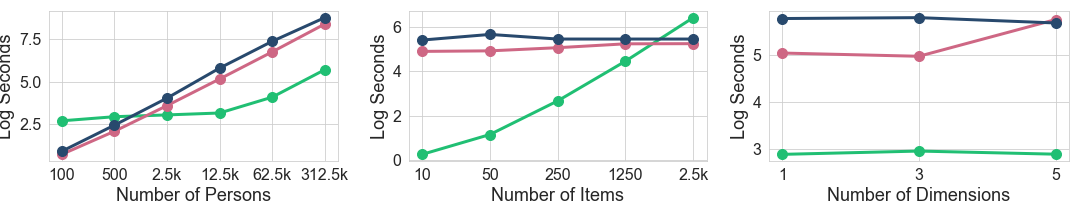
\includegraphics[width=\textwidth]{images/chapter7/ideal/all_cost.pdf}
    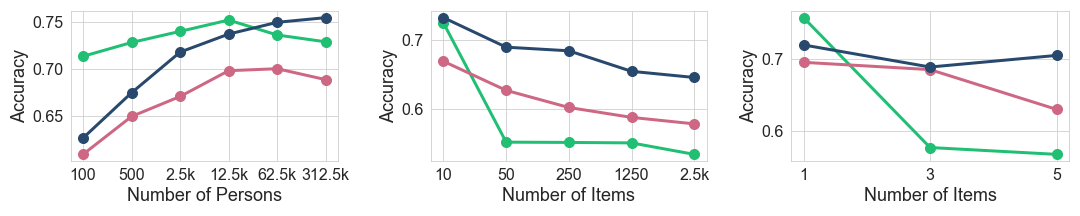
\includegraphics[width=\textwidth]{images/chapter7/ideal/all_acc.pdf}
    
\includegraphics[width=0.4\textwidth]{images/chapter7/ideal/legend.pdf}
    \caption{Performance of inference algorithms on synthetic data from an ``ideal point'' or unfolding IRT model, as we vary the number of people, items, and latent ability dimensions. (Top) Computational cost in log-seconds (e.g.~1 log second is about 3 seconds whereas 10 log seconds is 6.1 hours). (Bottom) Accuracy of held-out data imputation.}
    \label{fig:synth_ideal_results}
\end{figure}

Figure~\ref{fig:synth_ideal_results} uncovers many similar trends as in the 2PL-IRT synthetic experiments: (1) VIBO outperforms MLE on missing data imputation where uncertainty has proven to be helpful; (2) the cost of VIBO is roughly equivalent to MLE, but both are more expensive than EM; (3) the cost of EM grows exponentially beyond VIBO as the number of items increase; and (4) at larger scale, VIBO outperforms EM in data imputation. 
Unlike the 2PL-IRT synthetic experiments, we find EM to perform more competitively in the IDL setting. 
Figure~\ref{fig:synth_ideal_results} shows that when the number of people is low ($<$10k), EM surpasses VIBO and MLE in accuracy. 
% \ndg{I don't see this for items... they look pretty compareable}
% mw: whoops, i was staring at the wrong graph
However, as the number of people increases to large scale (e.g. 312.5k), EM again falls short of VIBO (and MLE). 
This is more pronounced when increasing the number of items: EM quickly degrades as items grow past 10. 
For 50 items, EM missing data imputation collapses to 55\% and approaches chance (50\%) as the number of items increases further.
While we also find decreasing accuracy for VIBO as the number of items increases, the drop is much smaller: from 73\% to 65\%.
Finally, as the number of dimensions grew from 1 to 5, whereas accuracy for EM decreases we find consistent performance for VIBO, one of the advantages of using a neural network.

\begin{figure}
    \begin{subfigure}[b]{0.5\textwidth}
        \centering
        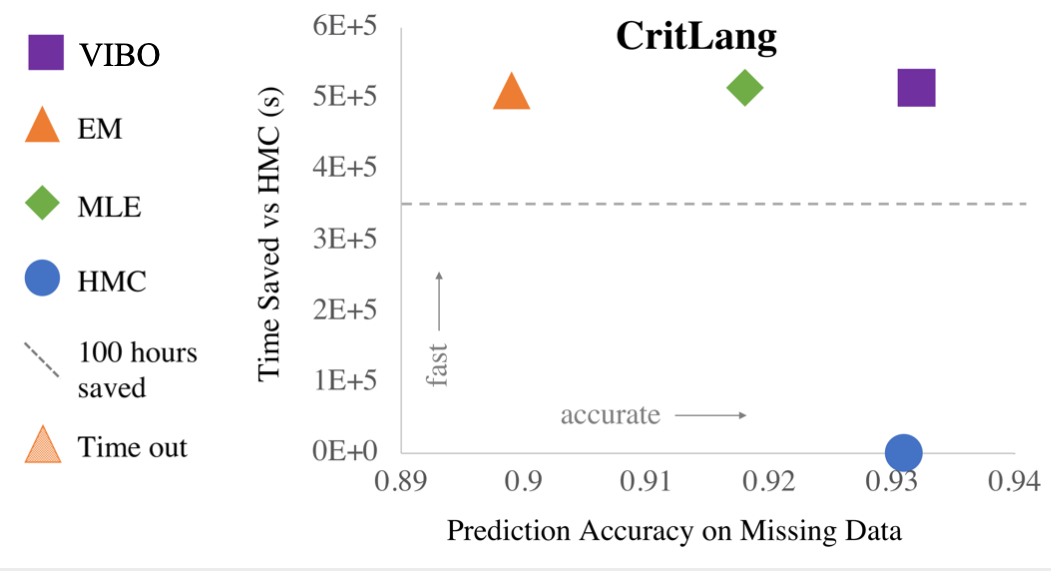
\includegraphics[width=\textwidth]{images/chapter7/excel/critlangacq.png}
        \caption{CritLangAcq}
    \end{subfigure}
    \begin{subfigure}[b]{0.5\textwidth}
        \centering
        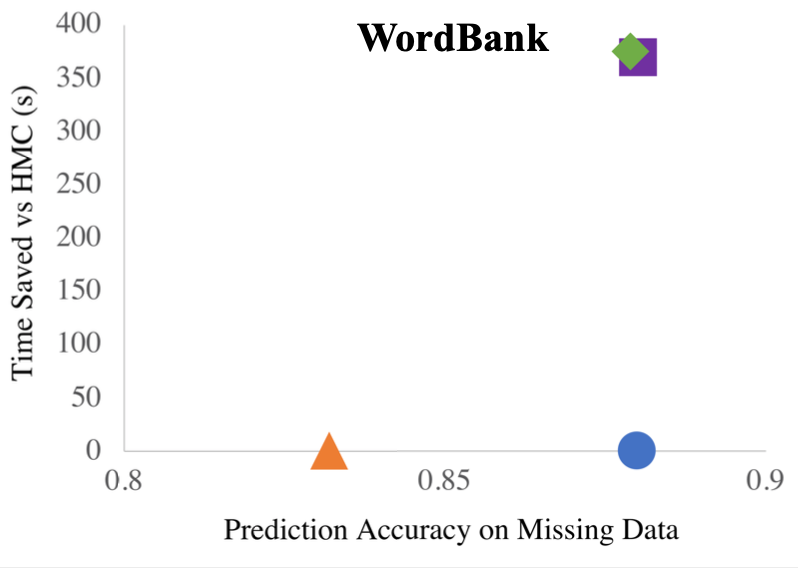
\includegraphics[width=0.75\textwidth]{images/chapter7/excel/wordbank.png}
        \caption{WordBank}
    \end{subfigure}
    \begin{subfigure}[b]{0.5\textwidth}
        \centering
        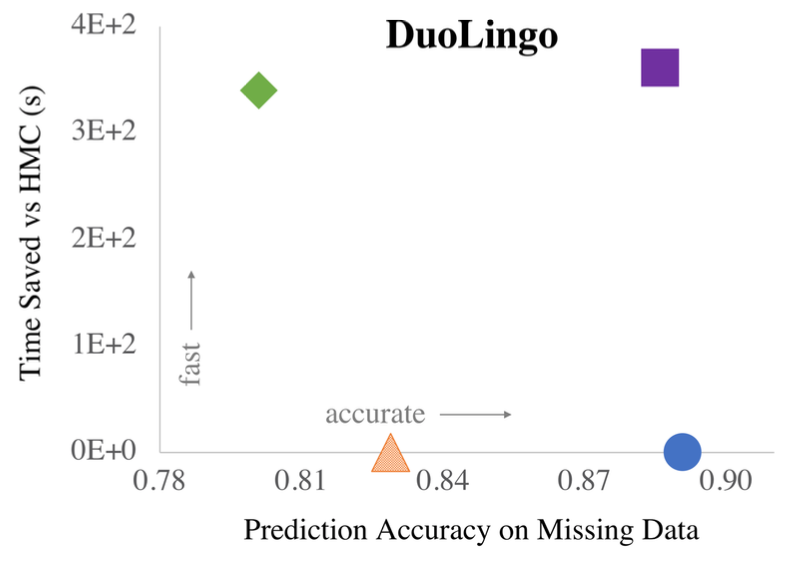
\includegraphics[width=0.75\textwidth]{images/chapter7/excel/duolingo.png}
        \caption{DuoLingo}
    \end{subfigure}
    \begin{subfigure}[b]{0.5\textwidth}
        \centering
        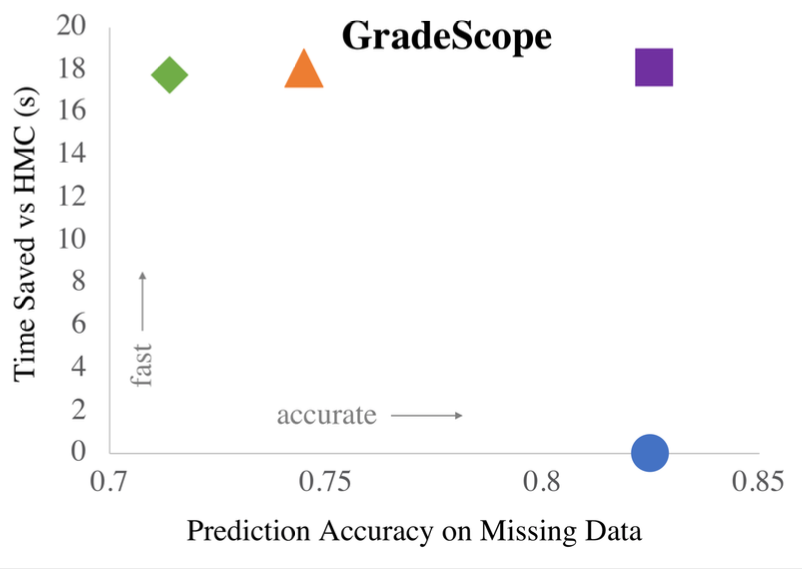
\includegraphics[width=0.75\textwidth]{images/chapter7/excel/gradescope.png}
        \caption{Gradescope}
    \end{subfigure}
    \begin{subfigure}[b]{0.5\textwidth}
        \centering
        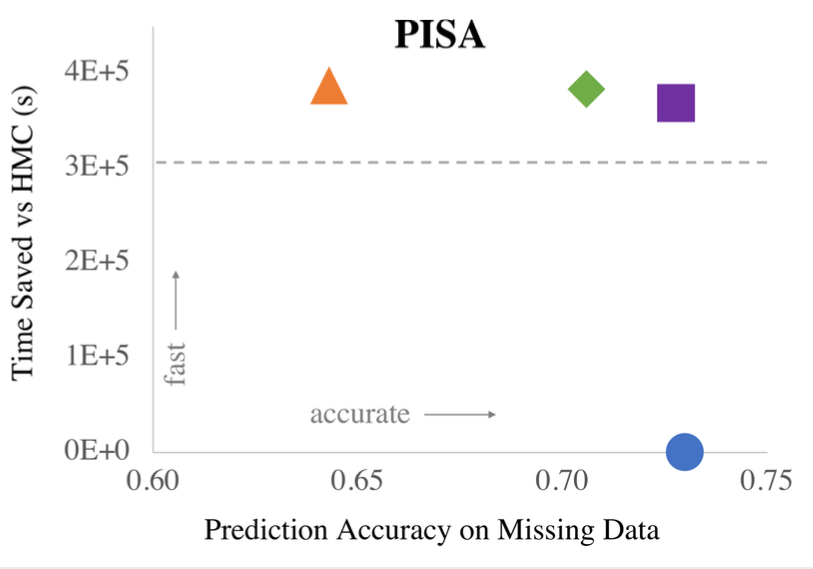
\includegraphics[width=0.75\textwidth]{images/chapter7/excel/pisa.png}
        \caption{PISA}
    \end{subfigure}
    \caption{Accuracy of missing data imputation for real world datasets plotted against time saved in seconds compared to using HMC.}
    \label{fig:realworld}
\end{figure}

\subsection{Real World Data Results}
We now apply VIBO to real world datasets in cognitive science and education.
Figure~\ref{fig:realworld} plots the  accuracy of imputing missing data against the time saved over HMC (the most expensive inference algorithm) for five  large-scale datasets.  
See Tables~\ref{table:realworld:cost} and \ref{table:realworld:acc} for a tabular representation.
% \bwd{i'd vote for numbers rather than shapes as points}
Points in the upper right corner are more desirable as they are both more accurate and faster.
The dotted line represents 100 hours saved compared to HMC.

\begin{table}
    \centering
    \caption{IRT Inference Cost (Log Seconds) on Real World Datasets}
    \label{table:realworld:cost}
    \small
    \begin{tabular}{lccccc}
    \hline
    Inference & CritLangAcq & WordBank & DuoLingo & Gradescope & PISA \\
    \hline
    MLE & \textbf{7.90} & \textbf{5.03} & 6.12 & 4.68 & 8.22 \\
    VIBO & 7.94 & 5.16 & \textbf{6.07} & 4.68 & 9.84 \\  
    EM & 8.81 & 6.52 & 7.65 & \textbf{2.57} & \textbf{6.11} \\
    HMC & 13.16 & 6.27 & 6.67 & 4.83 & 12.87 \\
    \hline
    \end{tabular}
\end{table}

\begin{table}
    \centering
    \caption{Missing Data Imputation on Real World Datasets}
    \label{table:realworld:acc}
    \small
    \begin{tabular}{lccccc}
    \hline
    Inference & CritLangAcq & WordBank & DuoLingo & Gradescope & PISA \\
    \hline
    MLE & 0.92 & 0.88 & 0.80 & 0.71 & 0.71 \\ 
    VIBO & \textbf{0.93} & \textbf{0.88} & \textbf{0.89} & \textbf{0.83} & \textbf{0.73} \\
    EM & 0.90 & 0.83 & 0.83 & 0.74 & 0.64 \\
    HMC & \textbf{0.93} & \textbf{0.88} & \textbf{0.89} & 0.82 & \textbf{0.73} \\
    \hline
    \end{tabular}
\end{table}

From Figure~\ref{fig:realworld}(a), we find many of the same patterns as we observed in the synthetic experiments.
Running HMC on CritLangAcq or PISA takes roughly 120 hours whereas VIBO takes 50 minutes for CritLangAcq and 5 hours for PISA, the latter being more expensive because of computation required for missing data.
In comparison, EM is sometimes faster than VIBO (e.g. Gradescope, PISA) and other times slower, depending on number of items.
With respect to accuracy, VIBO and HMC are again identical, outperforming EM by up to 8\% in missing data imputation.
Interestingly, we find the ``overfitting" of MLE to be more pronounced here.
If we focus on DuoLingo and Gradescope, the two datasets with pre-existing large portions of missing values, MLE is surpassed by EM, with VIBO achieving accuracies 10\% higher.

Another way of exploring a model's ability to explain data, for fully Bayesian models, is posterior predictive checks.
Figure~\ref{fig:realworld}(b) shows posterior predictive checks comparing VIBO and HMC.
We find that the two algorithms strongly agree about the average number of correct people and items in all datasets.
The only systematic deviations occur with DuoLingo: it is possible that this is a case where a more expressive posterior approximation would be useful in VIBO, since the number of items is greater than the number of people.

\begin{figure}
    \begin{subfigure}[b]{0.5\textwidth}
        \centering
        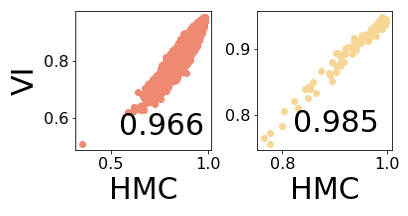
\includegraphics[width=0.75\textwidth]{images/chapter7/posterior_predictives/critlangacq.png}
        \caption{CritLangAcq}
    \end{subfigure}
    \begin{subfigure}[b]{0.5\textwidth}
        \centering
        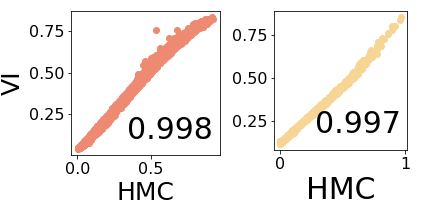
\includegraphics[width=0.75\textwidth]{images/chapter7/posterior_predictives/wordbank.png}
        \caption{WordBank}
    \end{subfigure}
    \begin{subfigure}[b]{0.5\textwidth}
        \centering
        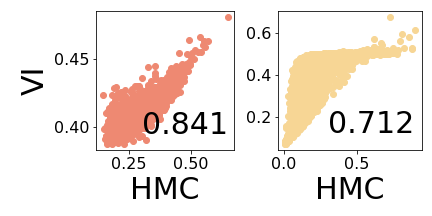
\includegraphics[width=0.75\textwidth]{images/chapter7/posterior_predictives/duolingo.png}
        \caption{DuoLingo}
    \end{subfigure}
    \begin{subfigure}[b]{0.5\textwidth}
        \centering
        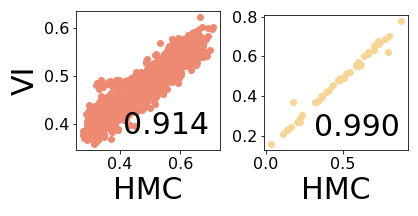
\includegraphics[width=0.75\textwidth]{images/chapter7/posterior_predictives/gradescope.png}
        \caption{Gradescope}
    \end{subfigure}
    \begin{subfigure}[b]{0.5\textwidth}
        \centering
        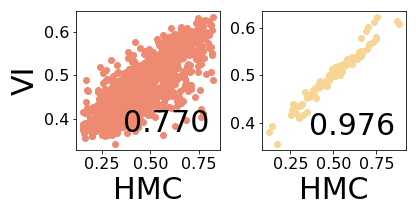
\includegraphics[width=0.75\textwidth]{images/chapter7/posterior_predictives/pisa.png}
        \caption{PISA}
    \end{subfigure}
    \caption{Samples statistics from the predictive posterior defined using HMC and VIBO. A correlation of 1.0 would be perfect alignment between two inference techniques. Subfigures in red show the average number of items answered correctly for each person. Subfigures in yellow show the average number of people who answered each item correctly.}
\end{figure}

\section{Deep Item Response Theory}
We have found VIBO to be fast and accurate for inference in 2PL-IRT, matching HMC in accuracy and EM in speed.
This classic IRT model is a surprisingly good model for item responses despite its simplicity.
Yet it makes strong assumptions about the interaction of factors, which may not capture the nuances of human cognition.
With the advent of much larger data sets we have the opportunity to explore corrections to classic IRT models, by introducing more flexible non-linearities.
As described above, a virtue of VI is the possibility of learning aspects of the generative model by optimizing the same inference objective.
We next explore several ways to incorporate learnable non-linearities in IRT, using the modern machinery of deep learning. 

\subsection{Nonlinear Generalizations of IRT}
In this section, we will use bolded notation to represent ability and item characteristics in multiple dimensions given the benefit of neural networks in higher dimensions. As a reminder, set $\textbf{a}_i = (a^{(1)}_i, \ldots, a^{(K)}_i )$, $\textbf{k}_j = (k^{(1)}_j, \ldots, k^{(K)}_j)$ for $K$ dimensions. We will still assume a 2PL model for exposition. To start, note we have assumed thus far that $p(r_{i,1:M}|\textbf{a}_i,\textbf{k}_{1:M}, d_{1:M})$ is a fixed IRT model defining the probability of a correct response to each item.
We now consider three different alternatives with varying levels of expressivity that help define a class of more powerful nonlinear IRT.

\subsubsection{Learning a Linking Function}
We replace the logistic function in standard IRT with a nonlinear linking function.
As such, it preserves the linear function for combining item and person characteristics, while generalizing the characteristic curves.
We call this VIBO (Link).
For person $i$ and item $j$, the 2PL-Link generative model is:
\begin{equation}
    p(r_{i,j}|\textbf{a}_i,\textbf{k}_j, d_j) =  f_\theta(-\textbf{a}_i^T \textbf{k}_j - d_j)
\end{equation}
where $f_\theta$ is a one-dimensional nonlinear function followed by a sigmoid to constrain the output to be within $[0,1]$.
In practice, we parameterize $f_\theta$ as a multilayer perceptron (MLP) with three layers of 64 hidden nodes with ELU nonlinearities.
Note that the standard IRT model is a special case when $f_\theta$ is the identity function.

\subsubsection{Learning a Nonlinear Interaction}$\quad$
Here, we no longer preserve the linear relationships between items and people and instead feed the ability and item characteristics directly into a neural network, which will combine the inputs nonlinearly.
We call this version VIBO (Deep).
For person $i$ and item $j$, the Deep generative model is:
\begin{equation}
    p(r_{i,j}|\textbf{a}_i, \textbf{k}_j, d_j) = f_\theta(\textbf{a}_i,\textbf{k}_j, d_j)
\end{equation}
where again $f_\theta$ includes a Sigmoid function at the end to preserve the correct output signatures.
This is an even more expressive model than VIBO (Link).
In practice, we parameterize $f_\theta$ as three MLPs, each with 3 layers of 64 nodes and ELU nonlinearities. 
The first MLP maps ability to a real vector; the second maps item characteristics to a real vector.
These two hidden vectors are concatenated and given to the final MLP, which outputs response probability.
While this model also includes standard IRT as a special case, it affords far more flexibility in how item characteristics and person abilities interact.

\subsubsection{Learning a Residual Correction}$\quad$
Although clearly a powerful model, we might fear that VIBO (Deep) becomes difficult to interpretable.
So, for the third and final nonlinear model, we use the standard IRT but add a nonlinear residual component that can correct for any inaccuracies.
We call this version VIBO (Residual).
For person $i$ and item $j$, the 2PL-Residual generative model is:
\begin{equation}
    p(r_{i,j}|\textbf{a}_i, \textbf{k}_j, d_j) = \frac{1}{1 + e^{-\textbf{a}^T_i\textbf{k}_j - d_j + f_\theta(\textbf{a}_i,\textbf{k}_j,d_j)}}
\end{equation}
During optimization, we initialize the weights of the residual network $f_\theta$ to 0, thus ensuring its initial output is 0.
This encourages the model to stay close to IRT, using the residual only when necessary.
We use the same architectures for the residual component as in VIBO (Deep).
% \ndg{it would be cool to explore the residuals learned by this model when we evaluate below... eg for what items does the residual differ most from zero? what do the corrections on the characteristic curves look like? (probably not necessary though) }

\subsubsection{Nonlinear IRT Evaluation}

A generative model explains the data better when it assigns observations higher probability.
We thus evaluate generative models by estimating the log marginal likelihood $\log p(\textbf{r}_{1:N,1:M})$ of the observed dataset.
A higher number (closer to 0) is better.
For a single individual, the log marginal likelihood of his or her $M$ responses can be computed as:
\begin{equation}
    \log p({r}_{i,1:M}) = \log \mathbf{E}_{q_\phi(\textbf{a}_i, \textbf{k}_{1:M}, d_{1:M}|{r}_{i,1:M})}\left[ \frac{p_\theta({r}_{i,1:M}, \textbf{a}_i, \textbf{k}_{1:M}, d_{1:M})}{q_\phi(\textbf{a}_i, \textbf{k}_{1:M}, d_{1:M}|{r}_{i,1:M})} \right]
    \label{eq:marg:evaluation}
\end{equation}
% \ndg{this equation is exact (not approx) as written, no? the approx comes from estimating with finite number of samples...}
We use 1000 samples to estimate Equation~\ref{eq:marg:evaluation}. 
As nonlinear models benefit from multi-dimensionality, we set $K=5$. All other hyperparameters are kept as in previous experiments.
We also measure accuracy on missing data imputation.
A more powerful generative model, that is more descriptive of the data, should be better at filling in missing values.
% \ndg{i don't think we say anywhere what latent dimension K we are using in these models? i assume it's the same in all models, but we should say explicitly. do we know how much the dimensionality matters?}
% \ndg{do we know how much the dimensionality matters?}
% \mwu{added below}

\subsubsection{Nonlinear IRT Results}
Table~\ref{table:real:nonlinear:loglike} compares the log likelihoods of observed data whereas Table~\ref{table:real:nonlinear:missing} compares the accuracy of imputing missing data.
We include VIBO inference with classical 1PL-IRT and 2PL-IRT generative models as baselines.
We find a consistent trend: the more powerful generative models achieve a higher log likelihood (closer to 0) and a higher accuracy.
In particular, we find very large increases in log likelihood moving from IRT to Link, spanning 100 to 500 log points depending on the dataset.
From Link to Deep and Residual, we find another increase of 100 to 200 log points.
In some cases, we find Residual to outperform Deep, though the two are equally parameterized, suggesting that initialization with IRT can find better local optima.
Improvements in log likelihood indicate the more flexible models can better model the distribution of responses.
In practice we often care about a particular aspect of this distribution: predictive accuracy.
The gains in log likelihood translate to a consistent 1 to 2\% increase in held-out accuracy for Link/Deep/Residual over IRT.

\begin{table}
    \caption{Log Likelihoods for Deep Generative IRT Models}
    \centering
    \tiny
    \begin{tabular}{lcccccc}
    \hline
    Model & CritLangAcq & WordBank & DuoLingo & Gradescope & PISA & TIMSS \\
    \hline
    Deep IRT & - & - & - & - & - & - \\
    VIBO (1PL-IRT) & $-11249.8 \pm 7.6$ & $-17047.2 \pm 4.3$ & $-2833.3 \pm 0.7$ & $-1090.7 \pm 2.9$ & $-13104.2 \pm 5.1$ & $-304.3 \pm 2.6$ \\
    VIBO (2PL-IRT) & $-10224.0 \pm 7.1$ & $-5882.5 \pm 0.8$ & $-2488.3 \pm 1.4$ & $-876.7 \pm 3.5$ & $-6169.5 \pm 4.8$ & $-282.7 \pm 4.0$ \\
    VIBO (IDL-IRT) & $-9841.2 \pm 3.8$ & $-8277.1 \pm 4.1$ & $-2158.5 \pm 1.1$ & $-1076.0 \pm 9.6$ & $-6068.3 \pm 2.3$ & $-462.3 \pm 3.8$ \ \\
    VIBO (LPE-IRT) & $-9902.1 \pm 5.5$ & $-6729.9 \pm 5.4$ & $-3217.2 \pm 4.4$ & $-833.4 \pm 2.9$ & $-6615.7 \pm 9.3$ & $-271.1 \pm 4.3$ \\
    VIBO (2PL-Link) & $-9590.3 \pm 2.1$ & $-5268.0 \pm 7.0$ & $-1833.9 \pm 0.3$ & $-750.8 \pm 0.1$ & $-6120.1 \pm 1.3$ & $-255.4 \pm 6.1$ \\
    VIBO (2PL-Deep) & $-9311.2 \pm 5.1$ & $\mathbf{-4658.4} \pm 3.9$ & $-1834.2 \pm 1.3$ & $\mathbf{-705.1} \pm 0.5$ & $-6030.2 \pm 3.3$ & $-237.2 \pm 3.3$ \\
    VIBO (2PL-Residual) & $\mathbf{-9254.1} \pm 4.8$ & $-4681.4 \pm 2.2$ & $\mathbf{-1745.4} \pm 4.7$ & $-715.3 \pm 2.7$ & $\mathbf{-5807.3} \pm 4.2$ & $\mathbf{-233.8} \pm 2.9$ \\
    \hline
    \end{tabular}
    \label{table:real:nonlinear:loglike}
\end{table}

\begin{table}
    \caption{Accuracy of Missing Data Imputation for Deep Generative IRT Models}
    \centering
    \scriptsize
    \begin{tabular}{lcccccc}
    \hline
    Model & CritLangAcq & WordBank & DuoLingo & Gradescope & PISA & TIMSS \\
    \hline
    Deep IRT & $0.934$ & $0.681$ & $0.884$ & $0.813$ & $0.524$ & $0.584$ \\
    VIBO (1PL-IRT) & $0.927$ & $0.876$ & $0.880$ & $0.820$ & $0.723$ & $0.756$ \\
    VIBO (2PL-IRT) & $0.932$ & $0.880$ & $0.886$ & $0.826$ & $0.728$ & $0.764$ \\
    VIBO (IDL-IRT) & $0.938$ & $0.856$ & $0.888$ & $0.818$ & $0.733$ & $0.582$ \\
    VIBO (LPE-IRT) & $0.938$ & $0.875$ & $0.855$ & $0.822$ & $0.706$ & $0.767$ \\
    VIBO (2PL-Link) & $0.945$ & $0.888$ & $0.891$ & $0.840$ & $0.718$ & $0.769$ \\
    VIBO (2PL-Deep) & $\mathbf{0.948}$ & $0.889$ & $\mathbf{0.897}$ & $0.847$ & $\mathbf{0.744}$ & $0.771$ \\
    VIBO (2PL-Residual) & $0.947$ & $\mathbf{0.889}$ & $0.894$ & $\mathbf{0.848}$ & $0.739$ & $\mathbf{0.775}$ \\
    \hline
    \end{tabular}
    \label{table:real:nonlinear:missing}
\end{table}

Next, we study the effect of dimensionality on nonlinear IRT. We hypothesized that by combining IRT with deep neural networks, high dimensional representations of ability and item characteristics would result in more powerful models with higher performance capabilities. Figure~\ref{fig:dimensionality} shows an experiment testing this hypothesis: we vary the dimensionality $K$ from 1 to 5 and find higher missing data accuracy (by almost 1\%) as $K$ increased from 1 to 3. Beyond $K=3$, the performance plateaus, showing smaller gains with higher dimensionality. Further, we see more dramatic increases in performance of VIBO (Deep) compared to VIBO (2PL).

We also compare our deep generative IRT models with a purely deep learning approach called Deep-IRT \cite{zhang2017dynamic} that does not model posterior uncertainty.
Unlike traditional IRT models, Deep-IRT was built for knowledge tracing and assumed sequential responses.
To make our datasets amenable to Deep-IRT, we assume an ordering of responses from $j=1$ to $j=M$.
As shown in Table~\ref{table:real:nonlinear:missing}, our models outperform Deep-IRT in all 5 datasets by as much as 30\% in missing data imputation.

\begin{figure}
    \centering
    \begin{subfigure}[b]{0.7\textwidth}
        \centering
        \includegraphics[width=\textwidth]{images/chapter7/dimensions/accuracy.pdf}
        \caption{Missing Data Accuracy}
    \end{subfigure}
    % \begin{subfigure}[b]{0.8\textwidth}
    %     \centering
    %     \includegraphics[width=\textwidth]{dimensions/loglike.pdf}
    %     \caption{Log Likelihood}
    % \end{subfigure}
    \caption{Effect of dimensionality $K$ on missing data imputation for VIBO (deep) and VIBO (2PL) on TIMSS. We observe decreasing gains from increasing dimensionality past $K=3$, and that  Deep outperforms 2PL at all dimensions.}
    \label{fig:dimensionality}
\end{figure}

We also include a baseline using VIBO inference with a IDL-IRT generative model that is capable of capturing nonlinearity through non-monotonic ICCs. 
Unlike deep generative IRT models, this assumes a specific nonlinear quadratic form. 
We find IDL to improve over a 2PL generative model but fall short of Deep and Residual models. 
Further, in WordBank or Gradescope, we find IDL to perform worse than a simpler 2PL model. 
% \ndg{???? i don't see this at all in the results. IDL is clearly worse than deep or residual.}
This diversity is not surprising given that the quadratic ICC adopted by IDL is a strong assumption that is not appropriate to all domains.
This speaks to the benefit of leveraging a neural network as the generative model: given data, it is flexible enough to adapt to any dataset without specifying the functional form ahead of time.
We next explore this flexibility in more detail.

\begin{figure}
    \centering
    \includegraphics[width=\textwidth]{images/chapter7/three_timss.pdf}
    \caption{Item characteristic curves (ICC) across six IRT models fit with VIBO on 3 questions from the TIMSS'07 mathematics test. The black line represents 1PL.}
    \label{fig:icc:timss}
\end{figure}

\subsection{Exploring the Flexibility of Response Curves} 

Traditionally, variations of IRT from 1PL to 2PL to LPE build progressively more complex models to map ability and item characteristics to probabilities of correctness. While early IRT models made simplifying assumptions about the world, newer IRT models sought to more faithfully represent the complexities of real world behavior using non-monotonicity, asymmetry, or other variations.
While we can continue to build progressively more complex IRT models, it is hard to believe that a single form can faithfully describe individuals across many domains. 
Rather, one of the primary benefits of VIBO is the ability to replace fixed IRT models with a deep generative model, parameterized by a neural network, that it can learn the appropriate mapping from ability and item characteristics to response probability. These neural networks produce meaningfully different IRT functions depending on the context.
To showcase this, we will show experiments visualizing ICCs in one, two, and then five dimensions.

\begin{table}
    \caption{Quality of fit on the TIMSS 2007 mathematics test Booklet 14. }
    % \ndg{why isn't vibo-link in this table? seems like a very relevant comparison!}}
    \label{table:timss:booklet}
    \begin{center}
    \begin{tabular}{lc}
    \hline
    Model & Log Likelhoods \\
    \hline
    % HMC & & -- \\
    VIBO (2PL-IRT) & $-306.42 \pm 4.1$ \\
    VIBO (3PL-IRT) & $-316.28 \pm 1.2$ \\
    VIBO (LPE-IRT) & $-274.50 \pm 4.0$ \\
    VIBO (Link-IRT) & $-264.01 \pm 4.7$ \\
    VIBO (2PL-Deep) & $-245.69 \pm 3.7$ \\
    VIBO (2PL-Residual) & $\mathbf{-243.55} \pm 1.8$ \\
    \hline
    \end{tabular}
    \end{center}
\end{table}

In one dimension, we fit the TIMSS response data with a 2PL, 3PL, and LPE IRT models to compare to three nonlinear IRT models: a learned linking function, a deep neural network, and a residual network as described above, using VIBO for inference in all cases. 
% Unlike in Figure~\ref{fig:residual_timss}, here we limit all models to one dimension to align with prior literature.
% \ndg{we should add vibo-link} % mwu - added
% There are 28 questions in booklet 14 with roughly 3.5k students. 
We visualize the ICCs captured by each of 5 IRT models on three questions (out of 28) in Figure~\ref{fig:icc:timss}, and report the log likelihood of the observed data in Table~\ref{table:timss:booklet}.
A higher number (closer to 0) in Table~\ref{table:timss:booklet} represents a better fit, summed over 28 questions. We find that while LPE has a significantly better fit than 2PL/3PL (a difference of 30 log points), we also find Deep and Residual to outperform LPE by another 30 log points -- a substantial difference. 
Analyzing Figure~\ref{fig:icc:timss}, we find that the nonlinear IRT models learn asymmetric ICCs, but are distinct from LPE curves. Further, the shape of the ICCs captured vary by question, showcasing the flexibility of neural networks. 

In two dimensions, we compare TIMSS response functions from VIBO (2PL) to VIBO (Deep) and VIBO (Residual) by visualizing the probability as level sets over the two ability features in Figure~\ref{fig:surfaces_timss} (3 random items shown). The contour lines vary from probability 0 to 1 of a correct response. 
We observe that while VIBO (2PL) has linear contours, VIBO (Deep) shows  curved contours that differ in shape by item. Furthermore, we find VIBO (Residual) to capture even more nonlinear behavior, represented by the jagged contours that again differ by item.
More research will be needed to understand which aspects of this non-linearity expose reliable psychometric effects.

\begin{figure}
    \centering
    \includegraphics[width=0.9\textwidth]{images/chapter7/three_2d_timess.pdf}
    \caption{Two dimensional response functions for three TIMSS questions. Each row depicts VIBO (2PL), VIBO (Deep), and VIBO (Residual) in order. }
    \label{fig:surfaces_timss}
\end{figure}

In five dimensions, we can again visualize the residuals captured by a deep generative model in Figure~\ref{fig:residual_timss} on TIMSS. To do this, we vary the ability from -5 to 5 across all 5 dimensions at once i.e., ability in every dimension is equal.
Interestingly, we find that the shape of the residuals differ by item and we see the ability to capture non-monotonic behavior as several of the red lines have sections that have near-zero slope. We also see that items cluster into distinct groups of response functions: some of them rapidly increase around ability -2 while others remain relatively flat until ability 0.
Compared to Figure~\ref{fig:icc:timss}, we find there ICCs are much less homogeneous as higher dimensionality allows neural networks to capture more expressive functions. 

\begin{figure}
    \centering
    \includegraphics[width=0.6\textwidth]{images/chapter7/residual/timss.pdf}
    \caption{Comparison of the item response function captured by VIBO (2PL) versus VIBO (Residual) over 28 items from the TIMSS dataset. The dotted black line represents the 2PL ICC curve -- which is the same across all questions -- while the red lines show the learned residuals to the ICC curve made by a deep neural network, which notably differ by item.}
    \label{fig:residual_timss}
\end{figure}

% \bwd{can we say anything about how our results look relative to the ones from lee and bolt? would be useful to note points of similarity as, to me, that wouuld be a huge selling point for our approach}
% \ndg{could say a little bit more about these results? eg thought the deep models could have been non-monotonic they aren't for these data -- because ability. maybe explain some big differences in ICCs between models? eg the first (top left) item in Fig 7.}
% \ndg{i'm not sure if we ever defined an ICC. make sure that;s somewhere above, or put it here...}
% \mwu{i dont think we need to for this crowd.}

\section{Extensions}

A substantial benefit of the variational Bayesian framework is allowing extensions with minimal changes to the core inference machinery. We illustrate an extension to the response model followed by another extension to the posterior.

\begin{table}[h!]
    \caption{Log Likelihoods with Polytomous Responses on DuoLingo}
    \label{table:duolingo:continuous}
    \begin{center}
    \begin{tabular}{lcc}
    \hline
    IRT Model & Train & Test \\
    \hline
    % HMC & & -- \\
    VIBO (2PL-IRT) &  $-22038.07$ & $-21582.03$ \\
    VIBO (2PL-Link) & $-17293.35$ & $-16588.06$ \\
    VIBO (2PL-Deep) & $\mathbf{-15349.84}$ & $\mathbf{-14972.66}$ \\
    VIBO (2PL-Residual) & $-15350.66$ & $-14996.27$ \\
    \hline
    \end{tabular}
    \end{center}
\end{table}

\begin{table}[h!]
    \caption{Missing Data Accuracy for Polytomous Responses on DuoLingo}
    \label{table:duolingo:polytomous}
    \begin{center}
        \begin{tabular}{lcc}
        \hline
        IRT Model & Binary & Polytomous (Rounded) \\
        \hline
        VIBO (2PL-IRT) & $0.886$ & $0.892$ \small{(+0.06)} \\
        VIBO (2PL-Link) & $0.891$ & $0.898$ \small{(+0.07)} \\
        VIBO (2PL-Deep) & $\mathbf{0.897}$ & $\mathbf{0.905}$ \small{(+0.08)} \\
        VIBO (2PL-Residual) & $0.894$ & $0.904$ \small{(+0.10)} \\
        \hline
        \end{tabular}
        \end{center}
\end{table}

\subsubsection{Polytomous Responses}
\label{sec:polytomous}
%Next, to showcase the generality of VIBO, we explore IRT over polytomous responses in a real world dataset. 
The DuoLingo corpus contains partial credit, computed as a fraction of times an individual translates a word correctly.
A more granular treatment of these polytomous values should yield a more faithful model that can better capture the differences between people.
We thus modeled the DuoLingo response data with generative models $p_\theta({r}_{i,1:M}|\textbf{a}_i, \textbf{k}_{1:M}, d_{1:M})$ similar to those used for binary data, but where the response distribution was a (truncated) Normal distribution with a fixed variance of 0.1. 
Table~\ref{table:duolingo:continuous} shows the log densities: we again observe large improvements from nonlinear models.
Furthermore, Table~\ref{table:duolingo:polytomous} compares missing data accuracy of VIBO on binary versus polytomous response data. For a fair comparison to the binary setting, we round the responses and predictions in the polytomous case. That is, a response of 0.3 and a prediction of 0.4 would be considered correct, whereas a response of 0.3 and a prediction of 0.7 would be incorrect. The results show that the IRT models trained on polytomous data outperform binary models consistently.
In this way, IRT can be extended to all kinds of response modalities (imagine students writing text, drawing pictures, or even coding), encouraging educators to assign open-ended work without having to give up proper tools of assessment.
% \ndg{do we have any way to compare these results to those from the binarized models? perhaps if we binarize the predictions of the continuous response model to look at held out accuracy?}

\begin{table}
    \caption{Effect of Richer Variational Posteriors on Log Likelihoods}
    \label{table:loglike:flows}
    \begin{center}
    \begin{tabular}{lcc}
    \hline
    Dataset & VIBO & VIBO-NF \\
    \hline
    CritLangAcq & $-10224.09$ & $-9945.30$ \\
    WordBank & $-5882.55$ & $-5510.67$ \\
    DuoLingo & $-2488.36$ & $-2174.10$\\
    Gradescope & $-876.75$ & $-800.68$ \\
    PISA & $-6169.55$ & $-5661.3$ \\
    \hline
    \end{tabular}
    \end{center}
\end{table}

\begin{table}
    \caption{Effect of Richer Variational Posteriors on Missing Data Accuracy}
    \label{table:accuracy:flows}
    \begin{center}
    \begin{tabular}{lcc}
    \hline
    Dataset & VIBO & VIBO-NF \\
    \hline
    CritLangAcq & $0.932$ & $0.940$ \small{(+0.08)} \\
    WordBank & $0.880$ & $0.889$ \small{(+0.09)}\\
    DuoLingo & $0.886$ & $0.886$ \small{(+0.00)}\\
    Gradescope & $0.826$ & $0.831$ \small{(+0.05)}\\
    PISA & $0.728$ & $0.741$ \small{(+0.13)} \\
    \hline
    \end{tabular}
    \end{center}
\end{table}

\subsubsection{Beyond Gaussian Posteriors}
So far, we have chosen the variational family $\mathcal{Q}$ to be Gaussian with diagonal covariance, mainly due to the benefits of reparameterization and product-of-experts.
However, for certain settings, such a simple family may not suffice.
If for example, the true posterior is multi-modal, our best Normal approximation will only capture one mode.
There is a rich body of work in the machine learning community dedicated to richer posterior distributions for variational inference \cite{rezende2014stochastic,tomczak2016improving,berg2018sylvester,kingma2016improved}.
To access a richer family of distributions, we consider the recent innovation of transforming samples from our Normal distribution to a more complex one using a \emph{normalizing flow}. 
In short, a ``flow'' is an invertible function with a tractable Jacobian determinant. 
If you compose several flows together, one can show that Gaussian samples can be mapped to samples from a richer, multimodal distribution. 
Critically, sampling remains differentiable through reparameterization.
Please refer to the Section~\ref{sec:app:vibo} for a detailed mathematical formulation.
We use the acronym VIBO-NF to refer to this generalized class of inference algorithms. 
% \ndg{i think perhaps all the math below should be moved to an appendix, instead having a short intuitive description here?}

Table~\ref{table:loglike:flows} shows results for a 2PL-IRT generative model. 
% \ndg{isn't it odd to use LL as the comparison metric here? since the model is fixed the asymptotic result of enough importance samples will be the same. maybe we want to look at accuracy as before? or at correlation with true params in the synthetic data case?}
We find that VIBO-NF has better log likelihoods across all datasets, often by hundreds of log points.
Similarly, Table~\ref{table:accuracy:flows} compares missing data accuracy between VIBO models with and without normalizing flows. We find a modest but consistent increase of 0.5 to 1 percent in performance. 
This preliminary evidence suggests that VIBO may benefit from more expressive posterior forms.

\section{Discussion and Conclusion}

\subsubsection{Limitations}

We describe one practical and one theoretical limitation of VIBO.
As a practitioner, these limitations are important to understand before use.

First, VIBO is sensitive to the length of training. Recall in the synthetic experiments that when using VIBO with limited number of people or items, it is important to increase the number of epochs for training to provide the model the opportunity to take more gradient steps (see left middle subplot in Figure~\ref{fig:synth_results}). 
Figure~\ref{fig:epoch} shows an experiment measuring the effect of number of epochs on the quality of parameter recovery in three synthetically generated datasets of size 100, 1000, and 10000. We observe that smaller datasets require more epochs as each epoch has fewer gradient steps (for a fixed batch size). For larger datasets, a single epoch may contain hundreds to thousands of gradient steps, requiring fewer epochs. (Note that total training time will be most determined by the total number of gradient steps.)
Unfortunately, optimal hyperparameters, like number of epochs, depend on the application and require some tuning. 
We thus recommend the practitioner monitor the results for convergence.

% we expect VIBO to have poor performance on small datasets, either limited in number of people or limited in number of items.
% Often, the inference networks (and generative models) in VIBO are parameterized by deep neural networks, which can have thousands to millions of trainable parameters.
% Sufficiently training these large networks necessitates large datasets. 
% Without sufficient examples, neural networks (and consequently VIBO) face challenges with poor generalization to new inference queries as well as overfitting to the training responses. 
% In such cases, we recommend the user to reduce the expressivity of the inference networks, minimizing the number of parameters.
% \ndg{i'm actually not sure this is true, as described. 'overfitting' to the observed people just yields the true params of the variational posterior for those ability variables (much like non-amortized VI). it's true that this won't generalize well to new people, but that isn't what IRT is usually used for or what we've evaluated. in contrast, under-parametrizing could have the effect of increasing the amortization gap, so i don't think we want to recommend it. overall, i don't actually understand what happens for small datasets -- or why vibo degraded with few people... }

Second, we note one unintended consequence of choosing a product-of-Gaussians as the form of the posterior.
Ideally, answering an easy question correctly should change a student's inferred ability less than answering a hard question correctly (and vice versa for hard questions).
%In the ideal scenario, if a student answers an easy question incorrectly but answers a hard question correctly, we would bias the inferred ability to be higher as a difficult question is more revealing of the student's true ability.
However, the product-of-experts posterior does not reflect this intuition, as a the Gaussian is symmetric. 
%VIBO would equally weight the easy and hard question.
While other families do exist that can reflect this asymmetry, there is not a closed form expression for a product of these components.
In theory, parameterizing the posterior $q(\textbf{a}_i|\textbf{d}_{1:M}, \textbf{r}_{i,1:M})$ as a recurrent neural network over any ordering of items $\{(\textbf{d}_j, \textbf{r}_{i,j})\}$ could alleviate this issue. 
See the Appendix for initial analysis and experiments comparing this ``Sequential VIBO'' versus the Product-of-Experts formulation of VIBO. 
These results suggest the product-of-Gaussians form is sufficient for the datasets we have used in this paper.
Future work should further investigate the advantages and disadvantages of more or less flexible parameterizations.
% Although normalizing flows do present one solution, future work can more carefully address this.
% \ndg{should decide if we want to add a quick experiment illustrating this? anyhow can describe the issue more clearly. would be good to say why we don't think this is ending up being a major issue for the experiments we ran...}

\subsubsection{When to use what?}
An outstanding question a practitioner might have after reading this paper is: \textit{which inference algorithm is best for what setting?}
Not wanting to add to the deluge of IRT strategies, we humbly suggest the following policy: If your data size is under 10k, use HMC or VIBO (or EM if speed is of utmost importance); if your data size is under 100k, use VIBO (or MLE if no data is missing and uncertainty is unimportant); anything beyond 100k, use VIBO and consider nonlinear IRT.
If you are working with multidimensional IRT, use VIBO or HMC. 
% \bwd{love it}

\subsubsection{Related Work}
\label{sec:related}

We described above a variety of methods for parameter estimation in IRT such as MLE, EM, and MCMC. The benefits and drawbacks of these methods are well-documented \cite{van2017handbook}, so we need not discuss them here. 
% \bwd{i would edit to read van der Linden for these cites}
Instead, we focus specifically on methods that utilize deep neural networks or variational inference to estimate IRT parameters.

While variational inference has been suggested as a promising alternative to other inference approaches for IRT \cite{van2017handbook}, there has been surprisingly little work in this area.
In an exploration of Bayesian prior choice for IRT estimation, \cite{natesan2016bayesian} posed a variational approximation to the posterior:
\begin{equation}
    p(\textbf{a}_i, \textbf{k}_j, d_j|r_{i,j}) \approx q_\phi(\textbf{a}_i, \textbf{k}_j, d_j) = q_\phi(\textbf{a}_i)q_\phi(\textbf{k}_j)q_\phi(d_j)
    \label{eq:natesan}
\end{equation}
This is an unamortized and independent posterior family, unlike VIBO.
Through ablations, we find both amortization and dependence of ability on items crucial.

We are aware of two approaches that incorporate deep neural networks into Item Response Theory: Deep-IRT \cite{yeung2019deep} and DIRT \cite{cheng2019dirt}. Deep-IRT is a modification of the Dynamic Key-Value Memory Network, or DKVMN \cite{zhang2017dynamic} that treats data as longitudinal, processing items one-at-a-time using a recurrent architecture. Deep-IRT produces point estimates of ability and item difficulty at each time step, which are then passed into a 1PL IRT function to produce the probability of answering the item correctly.
The main difference between DIRT and Deep-IRT is the choice of neural network: instead of the DKVMN, DIRT uses an LSTM with attention \cite{vaswani2017attention}.
In our experiments, we compare our approach to Deep-IRT and find that we outperform it by up to 30\% on the accuracy of missing response imputation.
On the other hand, our models do not capture the longitudinal aspect of response data.
Combining the two approaches would be natural.

Lastly, \cite{curi2019interpretable} used a VAE to estimate IRT parameters in a 28-question synthetic dataset.
However, this approach modeled ability as the only unknown variable, ignoring items.
Our analogue to the VAE builds on the IRT graphical model, incorporating both ability and item characteristics in a principled manner.
This could explain why \cite{curi2019interpretable} report the VAE requiring substantially more data to recover the true parameters when compared to MCMC whereas we find comparable data-efficiency between VIBO and MCMC.

\subsubsection{Conclusion}
Item Response Theory is a paradigm for reasoning about the scoring of tests, surveys, and similar measurement instruments.
Notably, the theory plays an important role in education, medicine, and psychology.
Inferring ability and item characteristics poses a technical challenge: balancing efficiency against accuracy.
Variational inference provides a potential solution, running orders of magnitude faster than MCMC algorithms while matching their state-of-the-art accuracy.

Many directions for future work suggest themselves.
First, further gains in speed and accuracy could be found by exploring different posterior families.
Second, more work is needed to understand deep generative IRT models and determine the most appropriate tradeoff between expressivity and interpretability.
% For instance, we found significant improvements from a learned linking function, yet in some applications monotonicity may be judged important to maintain -- greater ability, for instance, should correspond to greater chance of success.
Finally, VIBO should enable more coherent, fully Bayesian, exploration of very large and important datasets, such as PISA.
Recent advances within AI combined with new massive datasets have enabled advances in many domains.
We have given an example of this fruitful interaction for understanding humans based on their answers.